\documentclass[12pt]{article}

\usepackage[utf8]{inputenc}
\usepackage[a4paper, total={6in, 8in}, margin=0.5in]{geometry}
\usepackage{fancyhdr}
\usepackage[english]{babel}
\usepackage{longtable}
\usepackage{tikz}
\usepackage{graphicx}
\usepackage{multicol}
\usepackage[parfill]{parskip}


\renewcommand{\familydefault}{\sfdefault}

\pagestyle{fancy}
\fancyhf{}
\rhead{Unit 4, Pressure and Heat}
\lhead{Formulae Physics 1}

\begin{document}
\section*{Newton's Laws}
	\begin{enumerate}
		\item A body remains at rest, or in motion at a constant speed in a straight line, unless acted upon by a force. (Things don't move on their own, bodies are lazy)
		\item When a body is acted upon by a force, the time rate of change of its momentum equals the force. ($F=ma$)
		\item If two bodies exert forces on each other, these forces have the same magnitude but opposite directions. (If I push a thing that won't budge, it pushes back at me with the same magnitude, but opposite direction)
	\end{enumerate}
\section*{Gravity and Normal Forces}
	The force of gravity is given as $F=mg$. $g=9.82$ in Sweden.

	Normal forces are always perpendicular to the ground. On a level plane at rest this is equal to the force of gravity. These are \emph{not} counter forces according to Newton's 3rd law, since they act only on one object, not two separate  ones.
	%\subsection*{Law of Gravitation}
	%	\begin{multicols}{2}
	%		\[F=G \times \frac{m_{1} \times m_{2}}{r^{2}}\] \break \break
	%		Where $M_{1}$ and $m_{2}$ are the masses of the objects, such as the earth and moon, $r$ is the distance between them, and $G=6.67 \times 10^{-11} Nm^2 / kg^2$. F is the force attracting each body towards the other.
	%	\end{multicols}
%\section*{Hooke's Law}
	%\begin{multicols}{2}
	%	\[F = k \times \Delta l\] \break \break
	%	Where $F$ is the force pulling the spring, $\Delta l$ is the change in length of the spring, and $k$ is the spring constant, which is an intrinsic property of the spring and is measured in the unit $N/m$
	%\end{multicols}
\section*{Friction}
	\begin{multicols}{2}
		\[F_{f} = \mu \times F_{N}\] \break
		Where $F_f$ is the force of friction, $\mu$ is the coefficient of friction, and $F_N$ is the normal force.
	\end{multicols}

\section*{Motion Formulae}
	\begin{multicols}{2}
		\[\Delta s = v \times \Delta t\]
		\[\Delta v = a \times \Delta t\]
		\[\Delta s = v_0 t + \frac{at^2}{2}\]
		\[2 \times a \times \Delta s = v_{1}^2 - v_{0}^2\]
	\end{multicols}
	Where $\Delta s$ is change in position, $\Delta t$ is change in time, $\Delta v$ is change in velocity, $a$ is acceleration, $v$ is velocity, $t$ is time, $s$ is position, $g$ is $9.82 m/s^2$ (in Sweden).
%\section*{Trigonometry \& Tilted Planes}
	%\begin{multicols}{2}
	%	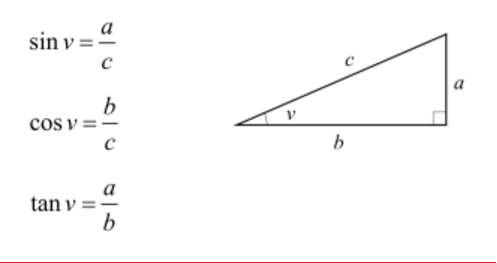
\includegraphics[width=5cm]{trig go brrrrrr.pdf}
	%	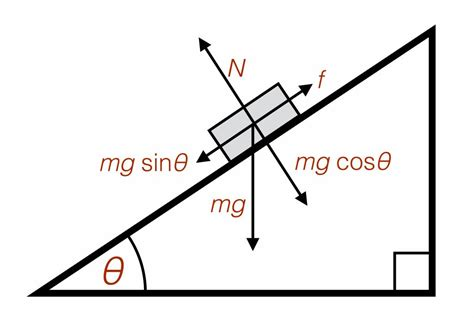
\includegraphics[width=5cm]{trianglefreebody.jpeg}
	%\end{multicols}
\section*{Energy}
	\begin{multicols}{2}
		\[W = F_{res} \times \Delta S\]
		\[\Delta E = W\]
		\[E_{p} = m g h\]
		\[E_{k} = \frac{m \times v ^2}{2}\]
		\[P = \frac{\Delta E}{\Delta t}\]
		\[\eta = \frac{\Delta E_{useful}}{\Delta E_{total}}= \frac{P_{useful}}{P_{total}} \]
		\[p = m \times v\]
		\[F \Delta t = \Delta p = mv_{2} - mv_{1}\]
	\end{multicols}
	Where $E$ is energy (J), $P$ is power (W), $\eta$ is efficieny, $p$ is momentum (kgm/s), $\Delta p$ is impulse (kgm/s) and W is work (Nm)
	\begin{multicols}{2}
		\subsection*{Energy Principle}
			Energy is always conserved, it is the same both before and after an event. \newline \break
		\subsection*{Conservation of Momentum}
			The sum of the momentum before and after a collsion always equal.
			\[p_{a1} + p_{b1} = p_{a2} + p_{b2}\]
	\end{multicols}
\section*{Pressure}
	\subsection*{Liquids}
		\begin{multicols}{2}
			\[p = \rho gh\] \break \break
			Where $p$ is the pressure, $\rho$ is the density of the liquid (), $g$ is the force downwards (In physics 1, $g = 9.82$), and $h$ is the depth.
		\end{multicols}
		\begin{multicols}{2}
			\[F_{lyft} = \rho gV\] \break \break
			Where $F_{lyft}$ is the force of lift, $\rho$ is the density of the liquid (or gas), $V$ is the volume of the submerged object, and $g$ is the force downwards (In physics 1, $g = 9.82$).
		\end{multicols}
	\subsection*{Ideal Gas Law}
		\begin{multicols}{2}
			\[ Pv = \eta RT \] \break
			Where $P$ is pressure in Pa, $v$ is volume in m³, $\eta$ is number of moles, $R$ is rate constant $R = 8.31451 J / mol K$, and $T$ is temperature (Kelvin).
		\end{multicols}
\section*{Heat}
	\begin{multicols}{2}
		\[ Q = cm \Delta T \] \break
		$Q$ is $\Delta E$, $c$ is specific heat capacity (4180 $K/kg \times K$ for water), $m$ is mass and $\Delta T$ is change in temp (Either C or K).
	\end{multicols}
	\begin{multicols}{2}
		\[ Q = l m \] \break
		$Q$ is $\Delta E$, $l$ is the energy required for one unit of mass to undergo the phase transition, and $m$ is the mass.
	\end{multicols}
	\begin{multicols}{2}
	\subsection*{Constants for water}
		$l = 2260000$ J/kg for boiling/condensation \newline
		$l = 330000$ J/kg for freezing/melting \newline
	\subsection*{Hot thing cold thing question}
		$-\Delta E_{thing 1} = \Delta E_{thing 2}$
	\end{multicols}
\end{document}
